\chapter{State of The Art}
\section{Virtual Counters}
Virtual Counters, or Guichets Virtuels in French, are online platforms that allow users to access services remotely without having to physically visit a location. They are designed to facilitate the interaction between users and service providers in a user-friendly, efficient and secure manner. The rise of digital technology has led to the development of various types of virtual counters, each with its own features and benefits.

\subsection{Types of Virtual Counters}
There are various types of virtual counters, such as:
\begin{itemize}
    \item \textbf{Web-based virtual counters:} These virtual counters are accessible through a web browser, and they allow users to access various online services offered by service providers.
    \item \textbf{Mobile-based virtual counters:} These virtual counters are accessible through mobile devices such as smartphones and tablets, and they offer users the convenience of accessing services on the go.
    \item \textbf{Kiosk-based virtual counters:} These virtual counters are installed in designated locations and allow users to access various services through self-service kiosks.
    \item \textbf{Chat-based virtual counters:} These virtual counters use instant messaging applications to facilitate communication between users and service providers, allowing users to access services through a chatbot or live chat.
\end{itemize}

\subsection{Examples of Virtual Counters}
Virtual counters have become increasingly popular in Algeria, and several organizations have adopted them to improve their services. Some examples of virtual counters in Algeria include:

\begin{itemize}
  \item \textbf{ElHanna:} The Caisse Nationale de l'Assurance Maladie (CNAS) in Algeria has created an application called "El Hanna" that allows its members to access various services related to their health insurance coverage, such as checking their eligibility for medical procedures, viewing their medical history
  \item \textbf{BaridiMob:} Algérie Poste has developed a virtual counter that allows customers to access their banking services online, such as transferring funds and paying bills.
  \item \textbf{Sonelgaz:} Sonelgaz has developed a virtual counter that allows customers to access their energy bills and make payments online.
  \item \textbf{E-Paiement:} E-Paiement is a mobile application developed by the Algerian government that allows citizens to pay bills, purchase government services, and access information using their mobile devices. The application is available for download on both Android and iOS devices.
\end{itemize}

Virtual counters have also been implemented in other countries, such as:

\begin{itemize}
  \item \textbf{eVisa:} The eVisa platform allows travelers to apply for visas online, reducing the need to physically visit an embassy or consulate.
  \item \textbf{eCNI:} The eCNI platform in France allows citizens to apply for their national identity cards online, reducing the need to visit a physical office.
\end{itemize}

In the next section, we will explore the benefits of virtual counters and their impact on the user experience.

\subsection{Benefits of Virtual Counters}
Virtual counters offer several benefits for both users and service providers. Some of the key benefits include:

\begin{itemize}
    
\item \textbf{Convenience:}  Virtual counters can be accessed from anywhere with an internet connection, making it more convenient for people to access services without having to physically go to a government office.
\item \textbf{Time-saving:} Virtual counters eliminate the need for users to physically visit a service center, saving them time and effort. Users can complete their transactions from the comfort of their own homes or offices, without having to wait in long lines or take time off work.
\item \textbf{Accessibility:} Virtual counters provide users with greater accessibility to services. They can access services from anywhere, at any time, as long as they have an internet connection. This is particularly beneficial for people with disabilities or those who live in remote areas and have limited access to physical service centers.
\item \textbf{Efficiency:} Virtual counters streamline the service delivery process by reducing paperwork, eliminating redundancies, and increasing transparency. This allows service providers to process transactions more efficiently and with greater accuracy.
\item \textbf{Cost-effective:} Virtual counters are typically more cost-effective for service providers than physical service centers. They require less physical infrastructure, fewer staff, and have lower operating costs. This can help service providers reduce costs and improve their bottom line.
\end{itemize}

\subsection{Challenges and Limitations}

Despite the benefits of virtual counters, there are also some challenges and limitations to consider. These include:
\begin{itemize}
    \item \textbf{Access and Connectivity}

One of the biggest challenges of virtual counters is ensuring that they are accessible to everyone, regardless of their location or technical ability. This requires reliable internet connectivity, as well as user-friendly interfaces and support for multiple languages.
\item \textbf{Security and Privacy}

Virtual counters also raise concerns about security and privacy. Users may be hesitant to share sensitive personal information online, and there is always the risk of data breaches or cyber attacks.
\item \textbf{Digital Divide}

Another limitation of virtual counters is the digital divide, which refers to the gap between those who have access to digital technologies and those who do not. This can be a particular challenge in developing countries or among low-income populations.
Technical Issues

Finally, virtual counters may also face technical issues such as server downtime, software bugs, or compatibility problems with different devices and platforms. These can all affect the user experience and the efficiency of the service.
\end{itemize}
Despite these challenges, virtual counters have the potential to revolutionize the way we access public services and interact with government agencies. By addressing these limitations, we can ensure that virtual counters are accessible, secure, and efficient for everyone.

\section{Introduction to CNAS Organization}
\subsection{Definition of CNAS organization}
The CNAS (Caisse Nationale des Assurances Sociales) is a public institution with specific management under Article 49 of Law No. 88-01 of January 12, 1988. It has legal personality and financial autonomy and is considered a merchant in its relations with third parties. The CNAS is responsible for managing social insurance benefits (illness, maternity, disability, and death), as well as occupational accidents and diseases (AO/D), and family allowances on behalf of the state. It also manages the collection, control, and litigation of contributions for financing benefits, as well as the management of the litigation related to the collection of subscriptions for financing rendered.

The CNAS assigns a national registration number to insured persons and employers and contributes to promoting the policy of prevention of AO/D and managing the AO/D prevention fund. It also manages benefits for beneficiaries of bilateral social security agreements, carries out medical control of beneficiaries, and undertakes actions to provide workers and their dependents with collective benefits in the form of health and social achievements. The CNAS also manages the aid and relief fund and concludes agreements with healthcare providers while ensuring the information of beneficiaries and employers.

The CNAS provides benefits to salaried workers, apprentices, job seekers, students, trainees in vocational training, disabled persons, veterans, social security beneficiaries (pensioners and annuitants), and beneficiaries of the lump sum solidarity allowance (sick, elderly and inactive persons). Dependents, including the spouse, minor children, unmarried inactive daughters, and dependent ascendants, are also eligible for benefits.

The CNAS covers healthcare and medication costs at 80\%, and in some cases 100\% (particularly for chronic diseases). Compensation for sick leave is 50\% of the salary for the first 15 days and is increased to 100\% of the salary beyond the 16th day, with a maximum duration of three years. Maternity benefits are fully covered, and working women are entitled to a 98-day maternity leave. The minimum amount of invalidity pensions is equal to 75\% of the guaranteed minimum wage. In the event of the insured person's death, a death benefit is paid to his or her dependents. Occupational risks are covered 100\% for healthcare and sick leave, and annuities are paid in the event of bodily harm or death resulting from occupational accidents or diseases.
\footnote{CNAS. (n.d.). Presentation of CNAS. Retrieved from \url{https://www.cnas.dz/}.}
\subsection{Organization of CNAS}
CNAS is managed by a Board of Directors and is under the supervision of the Minister of Labor, Employment and Social Security. Its headquarters is located in Algiers (BEN AKNOUN), and it has national jurisdiction with both central and local services.\footnote{CNAS. (n.d.). Presentation of CNAS. Retrieved from \url{https://www.cnas.dz/}.}

to fulfill its missions, CNAS has: 
\begin{itemize}
\item A General Directorate.
\item 49 provincial agencies (including 2 in Algiers).
\item 826 payment structures, including:
\begin{itemize}
\item 356 payment centers.
\item 401 payment branches.
\item 69 local correspondences.
\end{itemize}
\item 4 specialized clinics (pediatric heart surgery, orthopedics and rehabilitation, ENT, dental).
\item 4 regional centers for medical imaging.
\item 35 diagnostic and treatment centers.
\item 55 pharmaceutical offices.
\item 30 nurseries and kindergartens.
\item A printing house in Constantine.
\item A family social center in Ben Aknoun.
\end{itemize}

\textit{Source: CNAS website (\url{http://www.cnas.dz/})}

\subsection{CNAS Organigram}
the CNAS organigram is made up of various departments, subdivisions, and services that work together to manage CNAS operations and deliver services to its beneficiaries.

\textbf{Director:} This is the topmost position in the CNAS hierarchy and is responsible for overseeing all CNAS operations.

\textbf{Division of Benefits:} This department is responsible for managing CNAS' various benefit programs, including health, maternity, and disability benefits.

\textbf{Division of Administration and General Resources:} This department is responsible for managing CNAS' administrative operations, such as human resources, procurement, and general resource management.

\textbf{Data Processing Center:} This department is responsible for managing CNAS' information technology systems and infrastructure.

\textbf{Division of Recovery and Finance:} This department is responsible for managing CNAS' financial operations, including revenue collection and disbursement.

\textbf{Medical Control Division:} This department is responsible for monitoring and controlling the quality of medical services provided by CNAS.

\textbf{Contracting Service:} This department is responsible for managing CNAS' contracts with healthcare providers.

\textbf{Personnel Division:} This department is responsible for managing CNAS' human resources operations, including recruitment, training, and personnel records management.

\textbf{Statistics, Archives and Documentation Service:} This department is responsible for managing CNAS' data and document management systems.

\textbf{Recovery Division:} This department is responsible for collecting outstanding debts owed to CNAS.

\textbf{Medical Control Service:} This department is responsible for conducting medical audits and reviewing medical claims.

\textbf{Pharmacy Service:} This department is responsible for managing CNAS' pharmacy operations, including the provision of pharmaceutical services to CNAS beneficiaries.

\textbf{Conventions Service:} This department is responsible for managing CNAS' relationships with healthcare providers, including contract negotiations and payment processing.

\textbf{General Resources Division:} This department is responsible for managing CNAS' facilities, equipment, and other general resources.

\textbf{Internal Control Unit:} This department is responsible for ensuring compliance with CNAS policies and procedures.

\textbf{Prevention Service:} This department is responsible for promoting public health and disease prevention.

\textbf{Contentious Service:} This department is responsible for managing CNAS' legal affairs, including dispute resolution and litigation.

\textbf{Payment Structures:} This department is responsible for managing CNAS' payment processing systems.

\textbf{Realization Service:} This department is responsible for managing CNAS' development and construction projects.

\textbf{C.I.W.Q:} This is a service that is responsible for managing CNAS quality control.

\textbf{CHIFA Service:} This department is responsible for managing CNAS' maternal and child health services.

\textbf{Affiliation and Transfer Service:} This department is responsible for managing CNAS' beneficiary registration and transfer operations.

\textbf{CLRQP:} This department is responsible for managing CNAS' social and family benefits.

\textbf{Accounting Service:} This department is responsible for managing CNAS' accounting operations.

\textbf{Finance Service:} This department is responsible for managing CNAS' finance operations.

\textbf{Security Service:} This department is responsible for managing CNAS' security operations, including physical security and cybersecurity.

\textbf{Employer Control Service:} This department is responsible for monitoring employers' compliance with CNAS regulations.

\textbf{High-Risk Service:} This department is responsible for managing CNAS' high-risk cases.

\textbf{Legal Affairs Service:} This department is responsible for providing legal advice and support to CNAS.
\medskip

Here is the organigram : 
\begin{figure}[h]
  \centering
  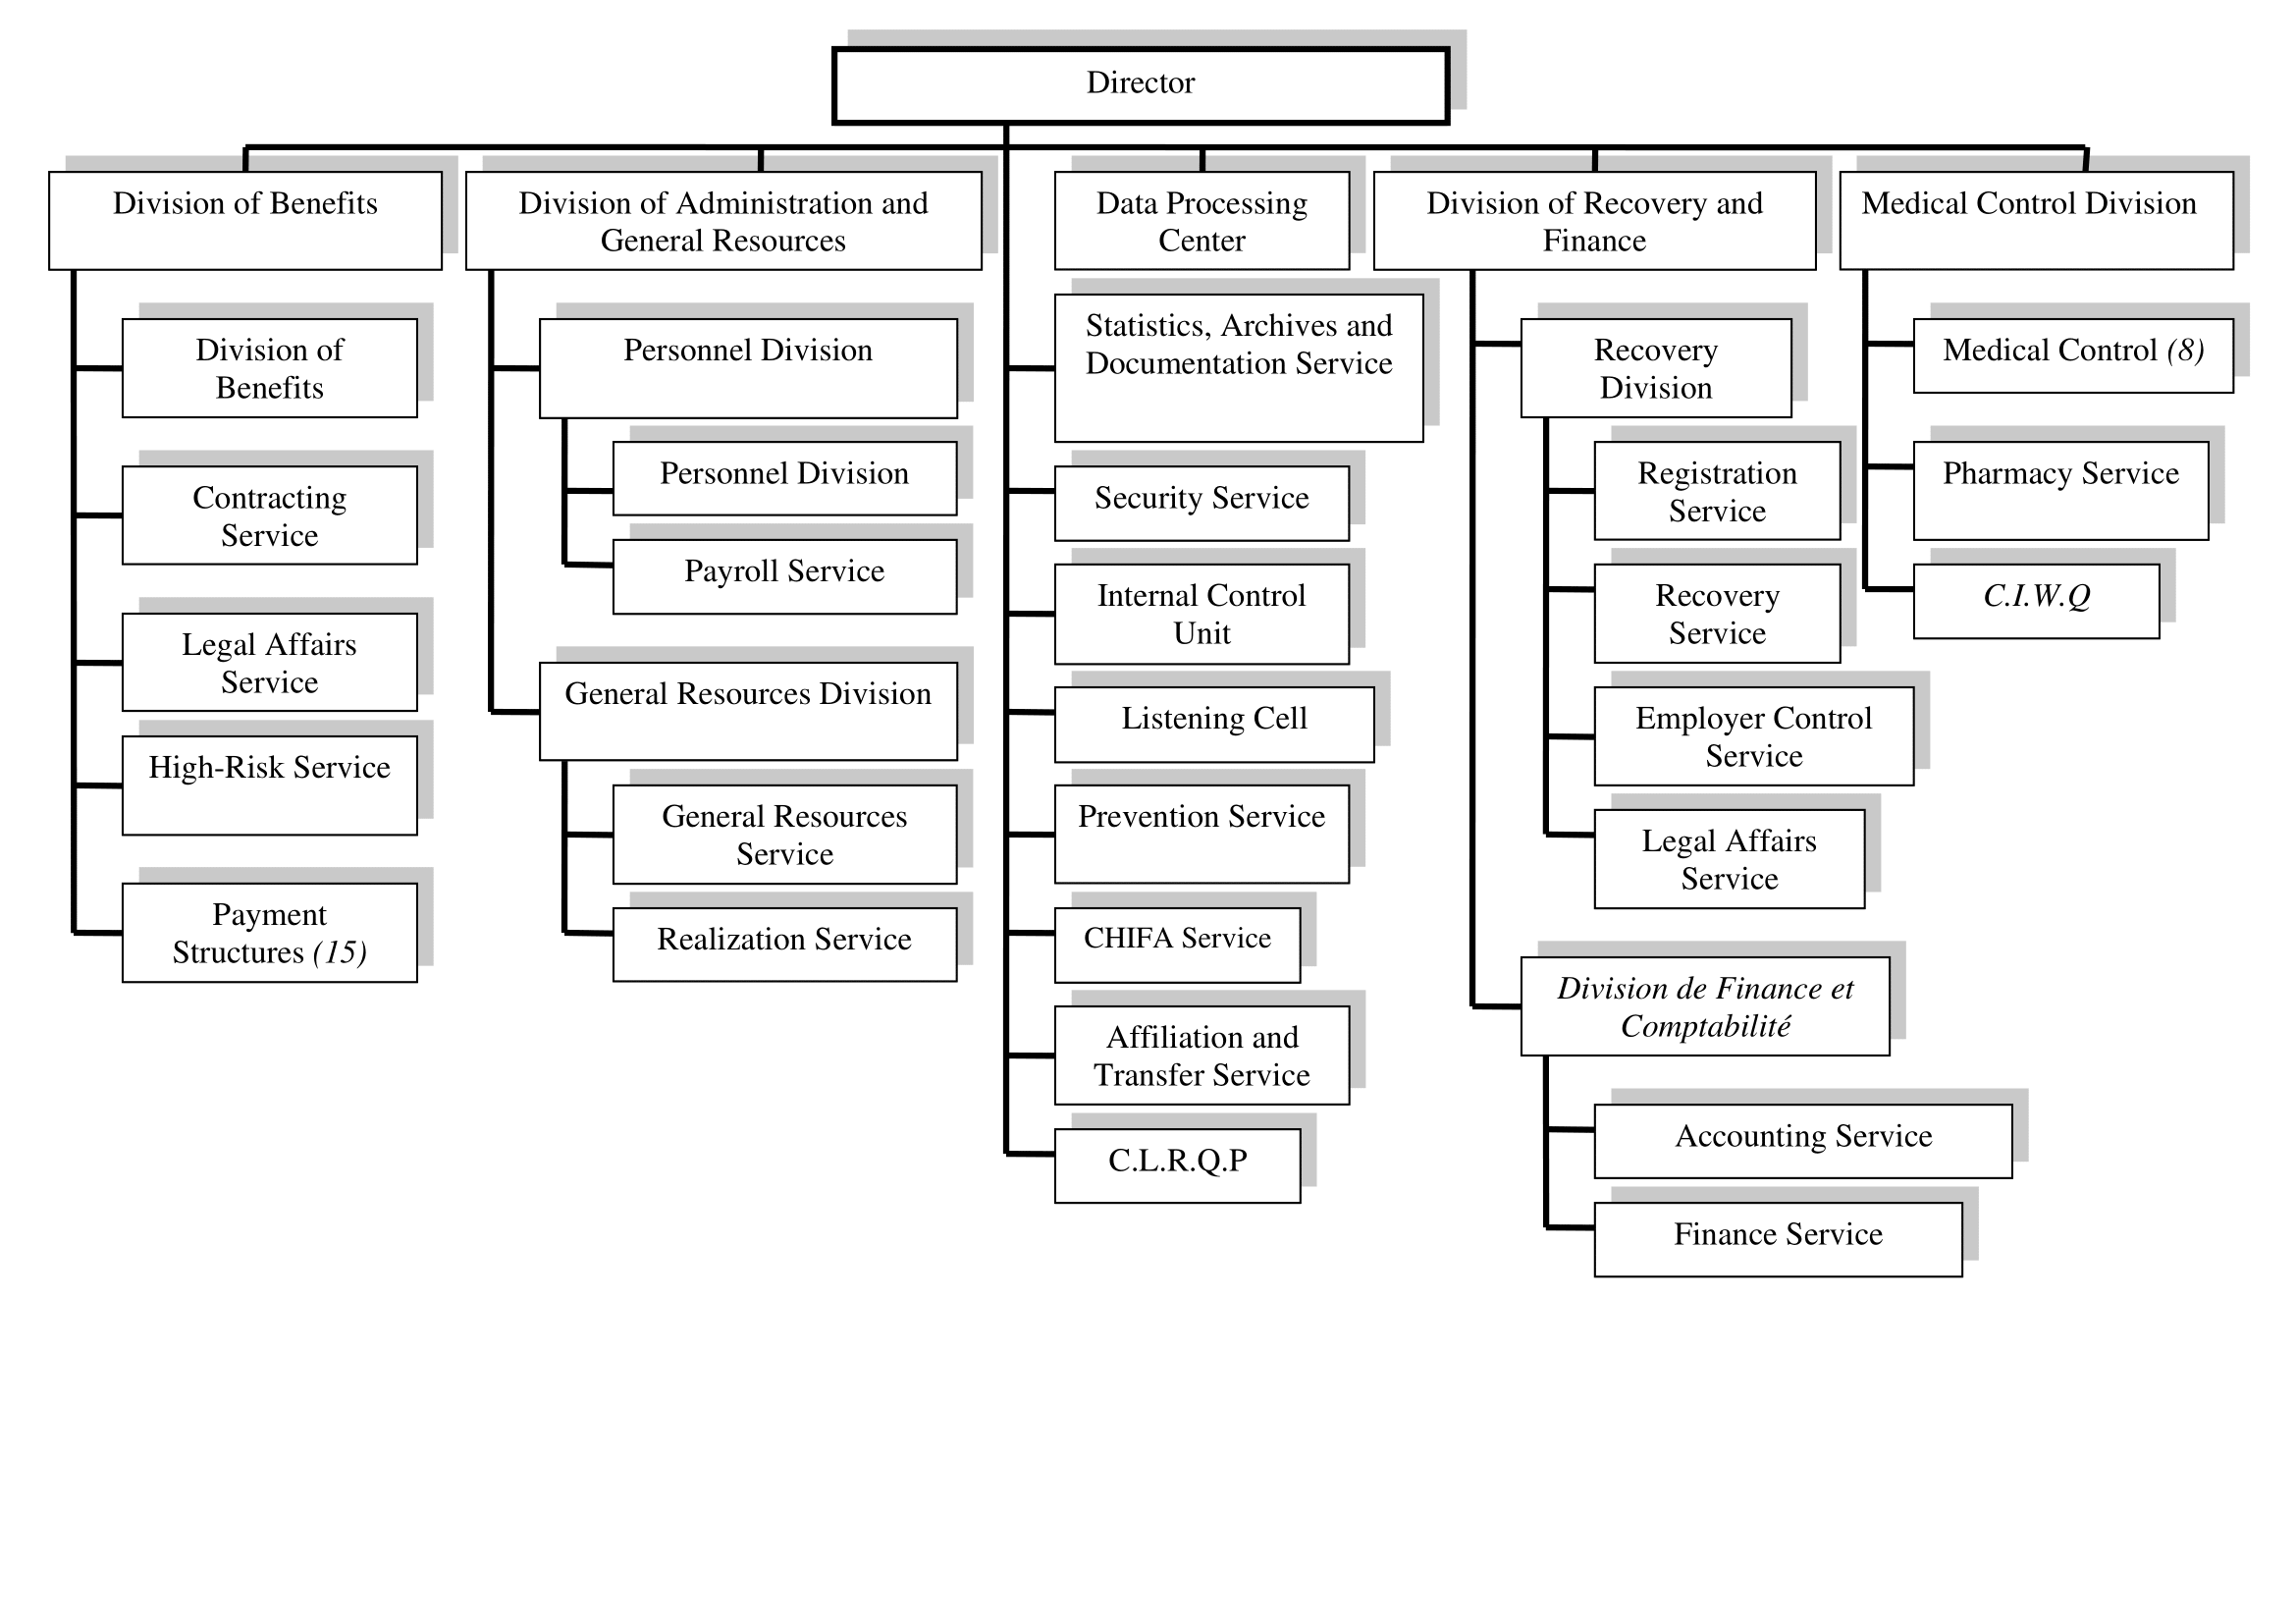
\includegraphics[width=1.0\textwidth]{organigram.png}
  \caption{Organigram of CNAS}
  \label{fig:organigram}
\end{figure}
\subsection{CNAS Services}
CNAS provides a range of services related to social security and healthcare to the Algerian population. These services include:
\begin{itemize}
    \item \textbf{Healthcare services:} CNAS operates its own specialized clinics and medical facilities, including four specialized clinics for cardiac surgery, orthopedics and rehabilitation, otorhinolaryngology, and dental care. It also runs 35 diagnostic and treatment centers, 55 pharmacies, and four regional medical imaging centers.

    \item \textbf{Social security services:} CNAS provides social security services to its members and their families, including health insurance, maternity leave benefits, disability benefits, and retirement pensions. It also offers services related to workplace safety and injury compensation.

    \item \textbf{Family services:} CNAS operates 30 nurseries and childcare centers to support working parents.

    \item \textbf{Payment services:} CNAS manages a network of payment centers and local correspondents to ensure the timely payment of social security benefits to its members.
\end{itemize}
\subsection{  Importance of CNAS services for the Algerian society}
These services are essential for the Algerian society, as they help provide access to healthcare and social security benefits to millions of people. CNAS's role in ensuring workplace safety and providing compensation for work-related injuries is also crucial in protecting the rights and wellbeing of workers across Algeria.
\section{Literature Review}
\label{sec:literature-review}

There has been a significant amount of research on the use of virtual counters in various contexts, including government services, healthcare, and banking.\footnote{Wang, Y., Wang, L., \& Wang, F. (2020). A review on virtual service counters. \textit{Journal of Service Science Research}, 12(1), 3-24.} Virtual counters have been found to offer several benefits, including improved efficiency, reduced wait times, and increased convenience for users.\footnote{Yao, Y., Yang, Q., \& Hu, Y. (2019). An evaluation of virtual counters in government services. \textit{International Journal of Public Administration}, 42(8), 708-721.}

One study found that virtual counters in government services were particularly effective in reducing wait times and improving the overall user experience.\footnote{Jia, J., \& Shi, Y. (2018). The impact of virtual service counters on customer satisfaction in government services. \textit{Public Administration Review}, 78(2), 239-250.} Another study focused specifically on virtual counters in healthcare and found that they could help reduce patient anxiety and improve the efficiency of healthcare services.\footnote{Liu, X., Li, Y., \& Chen, G. (2021). The impact of virtual service counters on patient satisfaction in healthcare. \textit{Journal of Healthcare Management}, 66(1), 24-34.}

In the banking industry, virtual counters have been used to provide personalized services to customers, such as financial advice and investment planning.\footnote{Zhu, Q., Chen, L., \& Fang, Y. (2019). The role of virtual service counters in enhancing customer satisfaction in the banking industry. \textit{International Journal of Bank Marketing}, 37(6), 1426-1442.} These services have been found to be effective in improving customer satisfaction and loyalty.

Overall, the literature suggests that virtual counters can offer significant benefits in a variety of contexts, including government services, healthcare, and banking. These benefits include improved efficiency, reduced wait times, and increased convenience for users. Based on this research, it is reasonable to expect that the implementation of a virtual counter system at CNAS could result in similar benefits for its users.

\section{Requirements analysis}
The requirements analysis phase identified several key features that the virtual counter for CNAS must provide. First, the system should provide a questionnaire for users to fill out, generating a checklist of necessary documents that must be obtained before the appointment. Second, it should allow users to book appointments online and provide them with a ticket number to avoid the need to wait in long queues. Third, it should allow CNAS staff to manage and monitor the appointments, including rescheduling or cancelling them if necessary. Fourth, the system should allow users to view their appointment history and provide feedback on their experience with the virtual counter. Finally, the system should ensure the security and privacy of all user data. These requirements will be used as a basis for the design, the conception and the implementation of the virtual counter system.

\section{Conclusion}
In this chapter, we have explored the current state of the art related to virtual counters, the organization of CNAS, and the literature review of virtual counters in various contexts. The use of virtual counters has been found to offer several benefits, including improved efficiency, reduced wait times, and increased convenience for users. CNAS, as an Algerian social security institution, provides a range of essential services to the Algerian society, including healthcare, childcare, and employment-related services.

Additionally, we have discussed the organization of CNAS and its numerous structures, such as its 49 Agences de wilaya and 826 structures de paiement, among others. Finally, we highlighted the importance of CNAS services for the Algerian society, emphasizing the need for modernization and innovation to ensure that these services continue to meet the evolving needs of its users.

Overall, this chapter provides a comprehensive understanding of the state of the art related to virtual counters and CNAS organization which serves as a foundation for the subsequent chapters in this dissertation.

